\section{Evaluation}
\label{sec:eval}

Our application, in addition to implementing our WiFi policies, would connect to a server and send a UDP packet every 100 milliseconds, stamped with a sequence number. To evaluate the performance our policies, we performed several experiments, with and without the appropriate policies enabled. For each experiment we inspected which packets were received to determine how many packets were dropped.

We present the setup and results from two experiments here. Each were inspired by the second and third problem situations presented. To test the Internet Access Testing policy, aproached a store with complimentary WiFi requireing authentication. For Predictive WiFi Abandonment, we left a WiFi network which was known to one of the authors to lost internet connectivity as a smartphone left [TODO: This is worded terribly][TODO: Better names for subsections...]

\subsection{Internet Access Testing - The Panera Test}
The problem of connecting to WiFi, without user intervention, that is unable to reach the internet is not cleanly measured. The impact of this issue varies on the users habits and the time spent within the network. To demonstrate this issue, as well as our solution we designed a realistic scenario to carry out. 

The experiment started across a parking lot, connected to AT\&T's HSPA network. We approached a store with public WiFi, which the phone would connect to once in range. Upon arriving at the door, we waited for 30 seconds and then attempted to access Google.com, waiting 10 seconds after successfully loading the page (including any delay from authentication).

\begin{figure}
	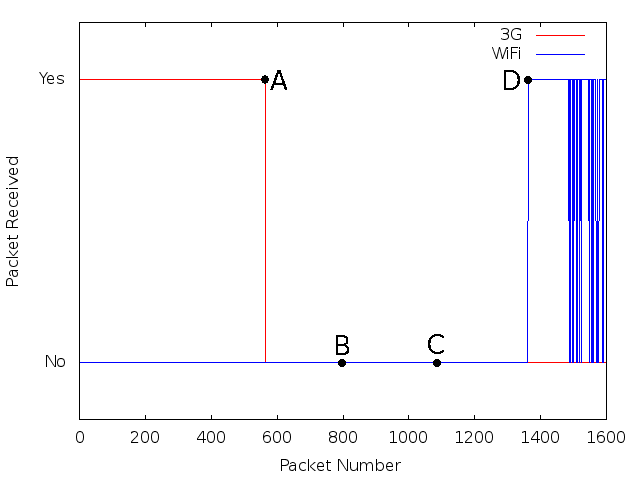
\includegraphics[width=0.5\textwidth]{paneraNoPolicy}
\end{figure}

Our server collected the UDP packets sent by the application allowing us 

\subsection{Predictive WiFi Abandonment - The Courtyards Test}
